\documentclass[11pt,a4paper]{article}
\usepackage[T1]{fontenc}
\usepackage[margin=22mm]{geometry}
\usepackage{amsmath,amssymb}
\usepackage{enumitem}
\usepackage{tikz}
\usetikzlibrary{arrows.meta,automata,positioning,shapes.geometric}
\usepackage{hyperref}
\hypersetup{hidelinks,pdftitle={Digital System Design -- Spring 2008 Midterm}}
\setlength{\parindent}{0pt}
\setlength{\parskip}{6pt}
\setlist[enumerate]{leftmargin=2em,itemsep=4pt,topsep=4pt}
\newcommand{\question}[2]{\subsection*{Question #1\hfill\normalfont #2}}
\begin{document}
\begin{center}
  {\LARGE\bfseries Digital System Design}\\[5pt]
  {\large Midterm (97/04/07)\\Spring 2008}\\[5pt]
  Total points: 105 points
\end{center}

\begin{quote}\small
\textbf{Transcription and provenance.} Source: \texttt{Final-Exam-2008-Answer.pdf}.
The title and date above are retained as printed, although the source filename
contains ``Final-Exam.'' Questions 1--2 are recoverable in full. The visible text
of Question 3 is retained on the next page, but its required circuit is cropped
in the supplied scan. The handwritten solution pages are not question content.
The state diagram is redrawn semantically with editable TikZ; its labels and
transitions are preserved. The numbered instructions below are quoted exam
content. Bracketed notes are editorial additions.
\end{quote}

\question{1}{20\%}
A sequential circuit with two D flip-flops, $A$ and $B$; two inputs, $x$ and
$y$; and one output, $z$, is specified by the following next-state and output
equations:
\[
\begin{aligned}
A(t+1)&=x'B+xy,\\
B(t+1)&=x'A,\\
Z&=AB.
\end{aligned}
\]
\begin{enumerate}[label=(\alph*)]
\item Draw the logic diagram of the circuit. (5\%)
\item List the state table for the sequential circuit. (15\%)
\end{enumerate}

\question{2}{20\%}
A state diagram with two state variables $D_A$ and $D_B$ and one output $z$
is shown in the following figure.
\begin{enumerate}[label=(\alph*)]
\item List the state table. (5\%)
\item Write down the maps of the two state variables $D_A$ and $D_B$ and the
output $z$; and then derive the Boolean equations for the three maps. (15\%)
\end{enumerate}

\begin{center}
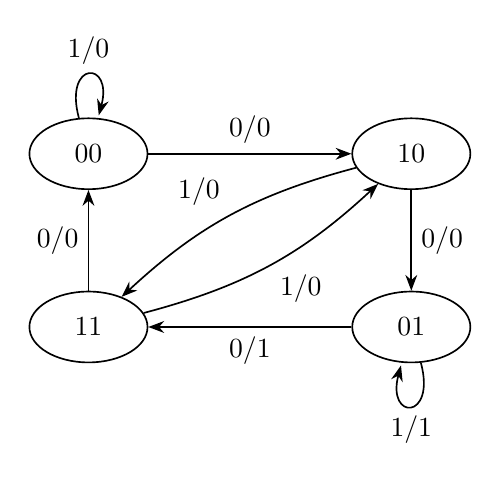
\begin{tikzpicture}[>=Stealth,semithick,
  state/.style={draw,ellipse,minimum width=15mm,minimum height=9mm},
  every edge/.style={draw,->},every edge quotes/.style={font=\small}]
  \node[state] (s00) at (0,2.2) {$00$};
  \node[state] (s10) at (4.1,2.2) {$10$};
  \node[state] (s11) at (0,0) {$11$};
  \node[state] (s01) at (4.1,0) {$01$};
  \path[->]
    (s00) edge[loop above] node {$1/0$} (s00)
    (s00) edge node[above] {$0/0$} (s10)
    (s10) edge node[right] {$0/0$} (s01)
    (s01) edge node[below] {$0/1$} (s11)
    (s11) edge node[left] {$0/0$} (s00)
    (s10) edge[bend right=14] node[above left] {$1/0$} (s11)
    (s11) edge[bend right=14] node[below right] {$1/0$} (s10)
    (s01) edge[loop below] node {$1/1$} (s01);
\end{tikzpicture}

Fig. 1. State diagram
\end{center}
{\small [Editorial note: all eight arrow labels are reproduced from the scan.
No initial-state arrow is shown in the original.]}

\newpage
\question{3}{10\% -- incomplete source figure}
\textbf{[Editorial note: the statement below is legible, but Fig. 2 is cropped.
This question is preserved as an incomplete excerpt and cannot be uniquely
answered from this source.]}

Given the circuit connected as shown in Fig. 2, assume that the wire delay is
not considered and the D flip-flop has setup time of 2 ns and hold time of
1 ns.
\begin{enumerate}[label=(\alph*)]
\item If the gate delay of the ``combinational logic 1'' is 12 ns and the gate
delay of the ``combinational logic 2'' is 5 ns, what is the minimum clock
period of this circuit to have normal operation? (5\%)
\item If ``combinational logic 1'' and ``combinational logic 2'' are both
replaced by the same new logic block with minimum delay requirement, what
is the minimum clock period of the new circuit to have normal operation?
(5\%)
\end{enumerate}

\begin{center}
\fbox{\parbox{0.82\linewidth}{\small
\textbf{Fig. 2 -- required circuit not recoverable.} Only part of a block
labelled ``Combinational Logic 2'' and portions of adjacent wires are visible.
The flip-flops, full connectivity and clock information lie outside the
supplied crop. No missing circuit is inferred from the handwritten answers.
}}
\end{center}

\vfill
{\small\textbf{Source completeness.} The printed total is 105 points. The
recoverable Questions 1--2 account for 40\%, and the visible but incomplete
Question 3 accounts for 10\%. No additional original question statements are
visible in the supplied PDF; the remaining pages contain handwritten answers.
This document therefore does not claim to reproduce a complete 105-point exam.}
\end{document}
